% ---------------------------------------------------------------
% Appendix: Supplementary Diagrams
% ---------------------------------------------------------------
\section{Supplementary Diagrams}
\label{sec:appendix}

This appendix contains entity-relationship and sequence diagrams that supplement the architecture description in Section~\ref{sec:arch}.

\subsection{Entity-Relationship Diagram}
\label{app:erd}

\begin{figure}[H]
  \centering
  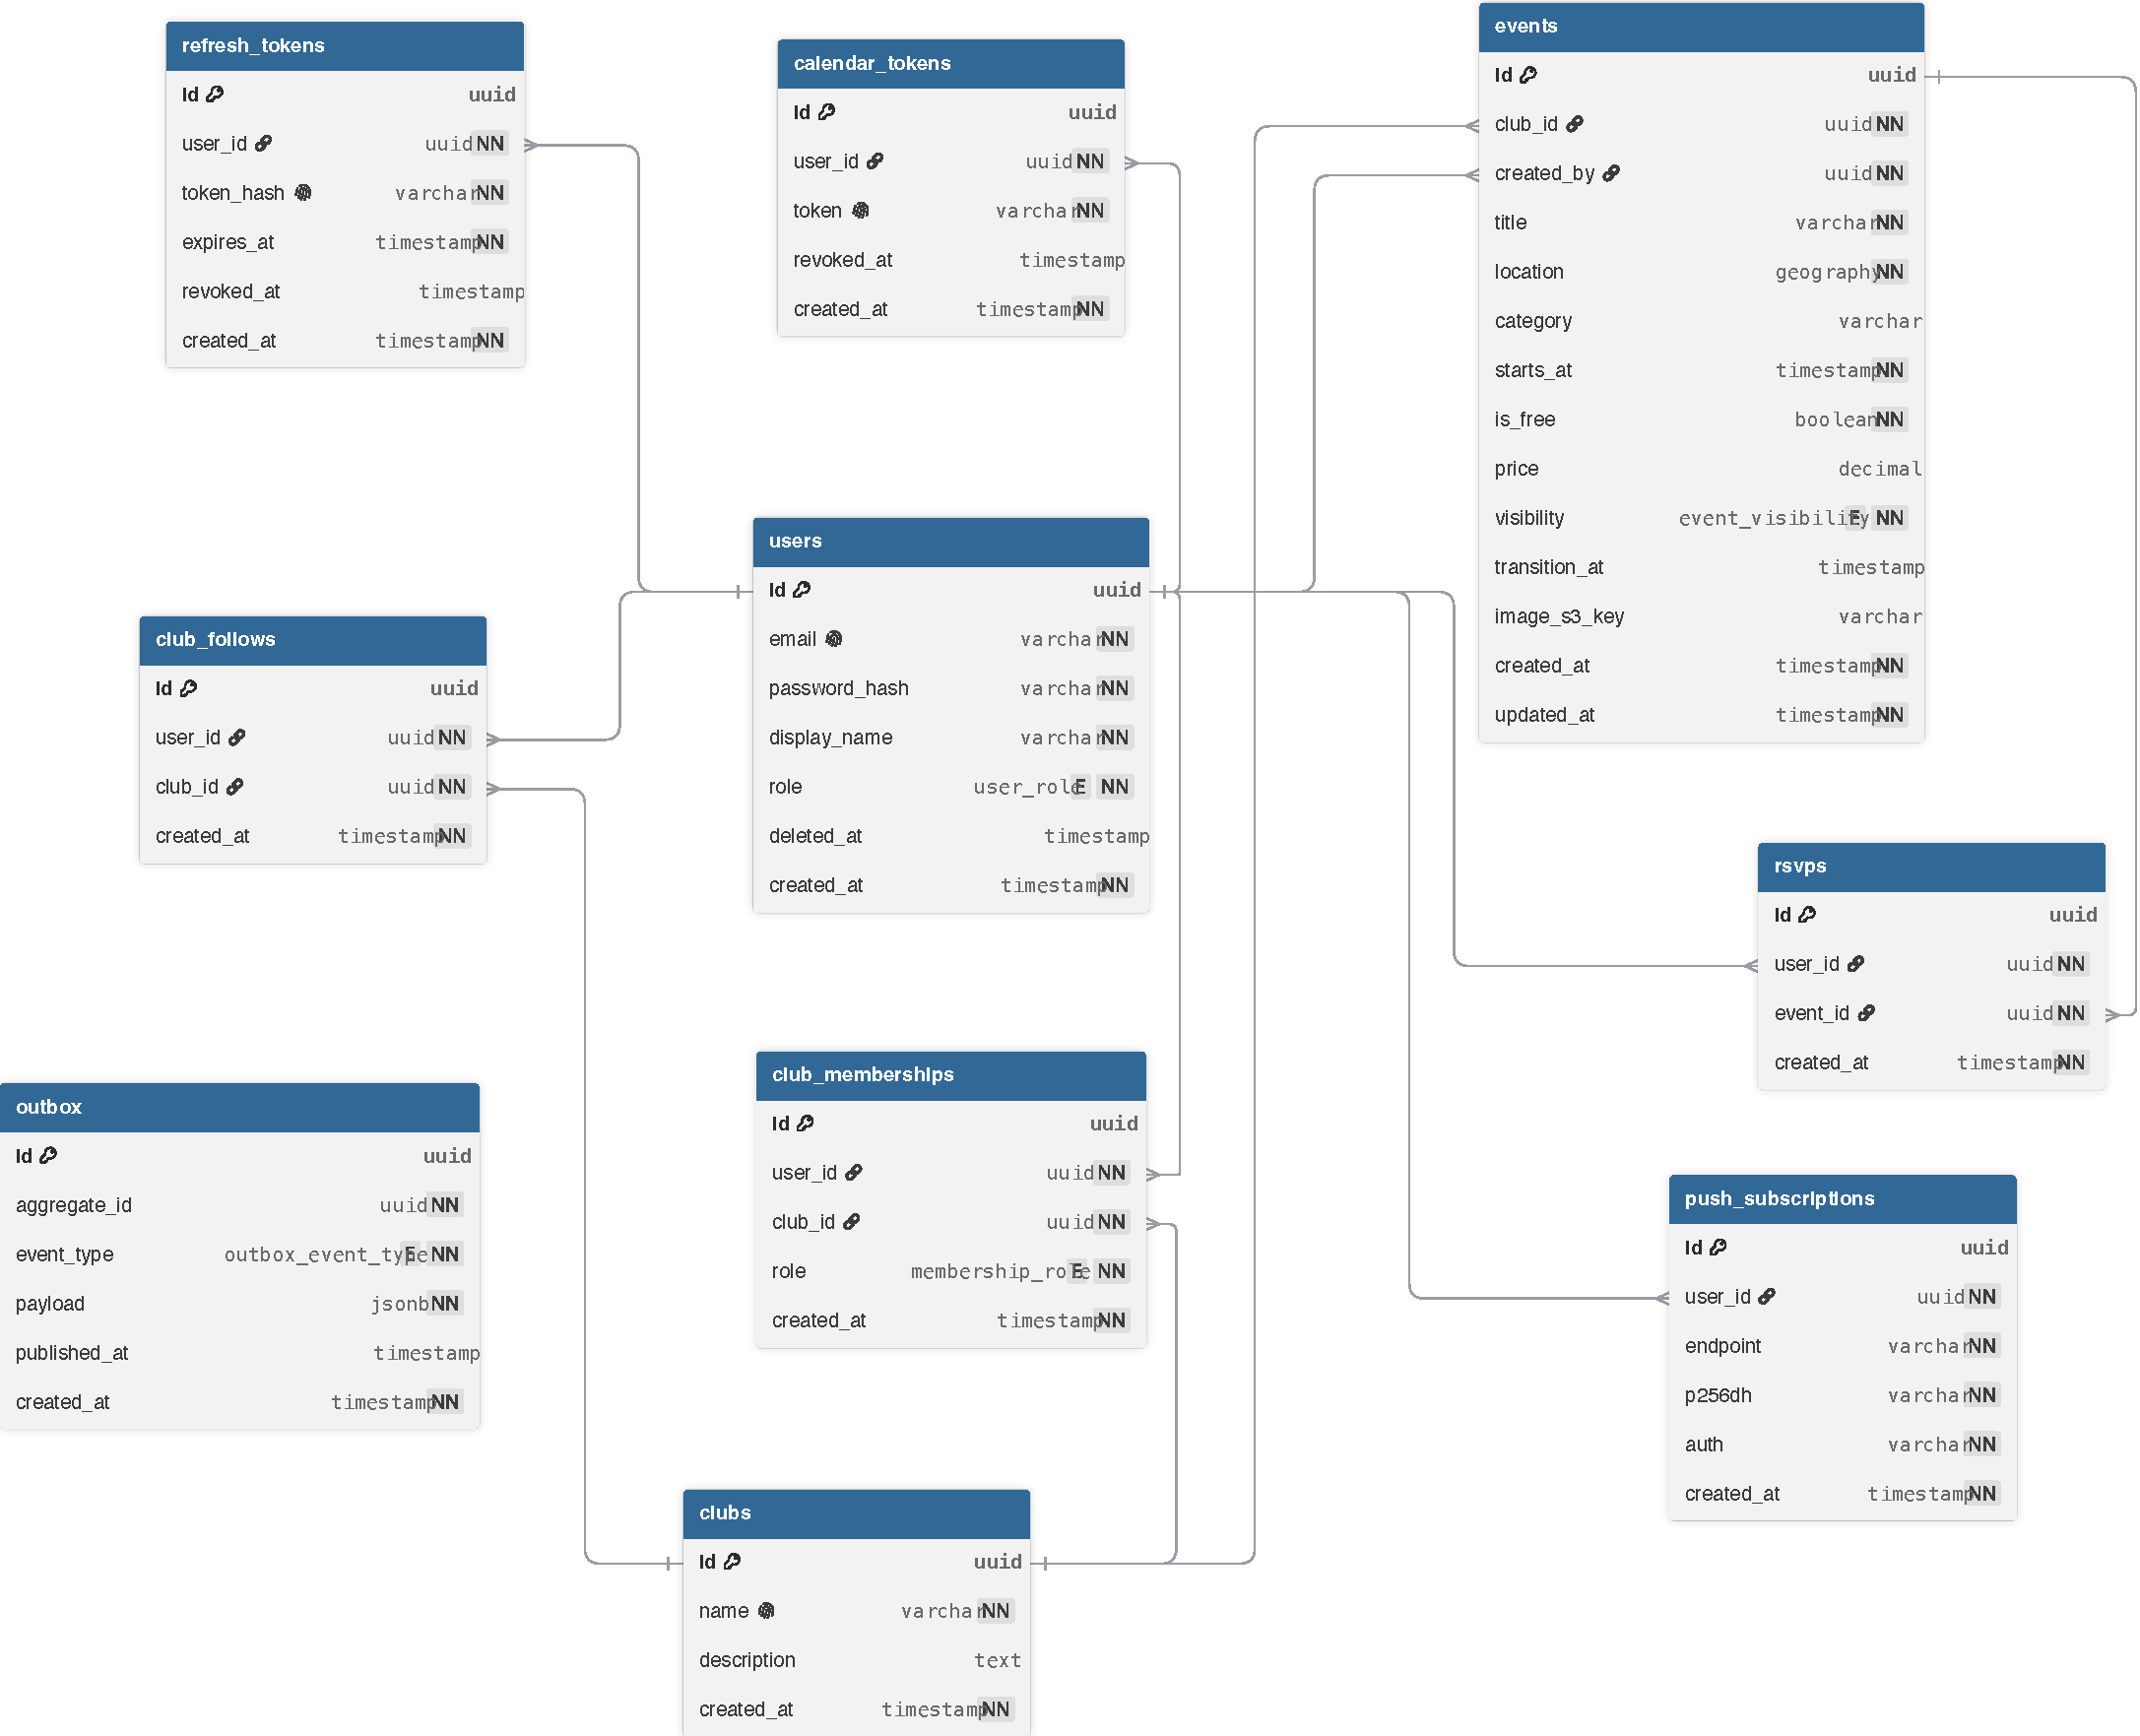
\includegraphics[width=\linewidth,height=0.85\textheight,keepaspectratio]{figures/erd.pdf}
  \caption{Database entity-relationship model showing the main tables and their relationships across bounded modules.}
  \label{fig:erd}
\end{figure}

\clearpage

\subsection{Sequence Diagram: RSVP Placement}
\label{app:seq:rsvp}

\begin{figure}[H]
  \centering
  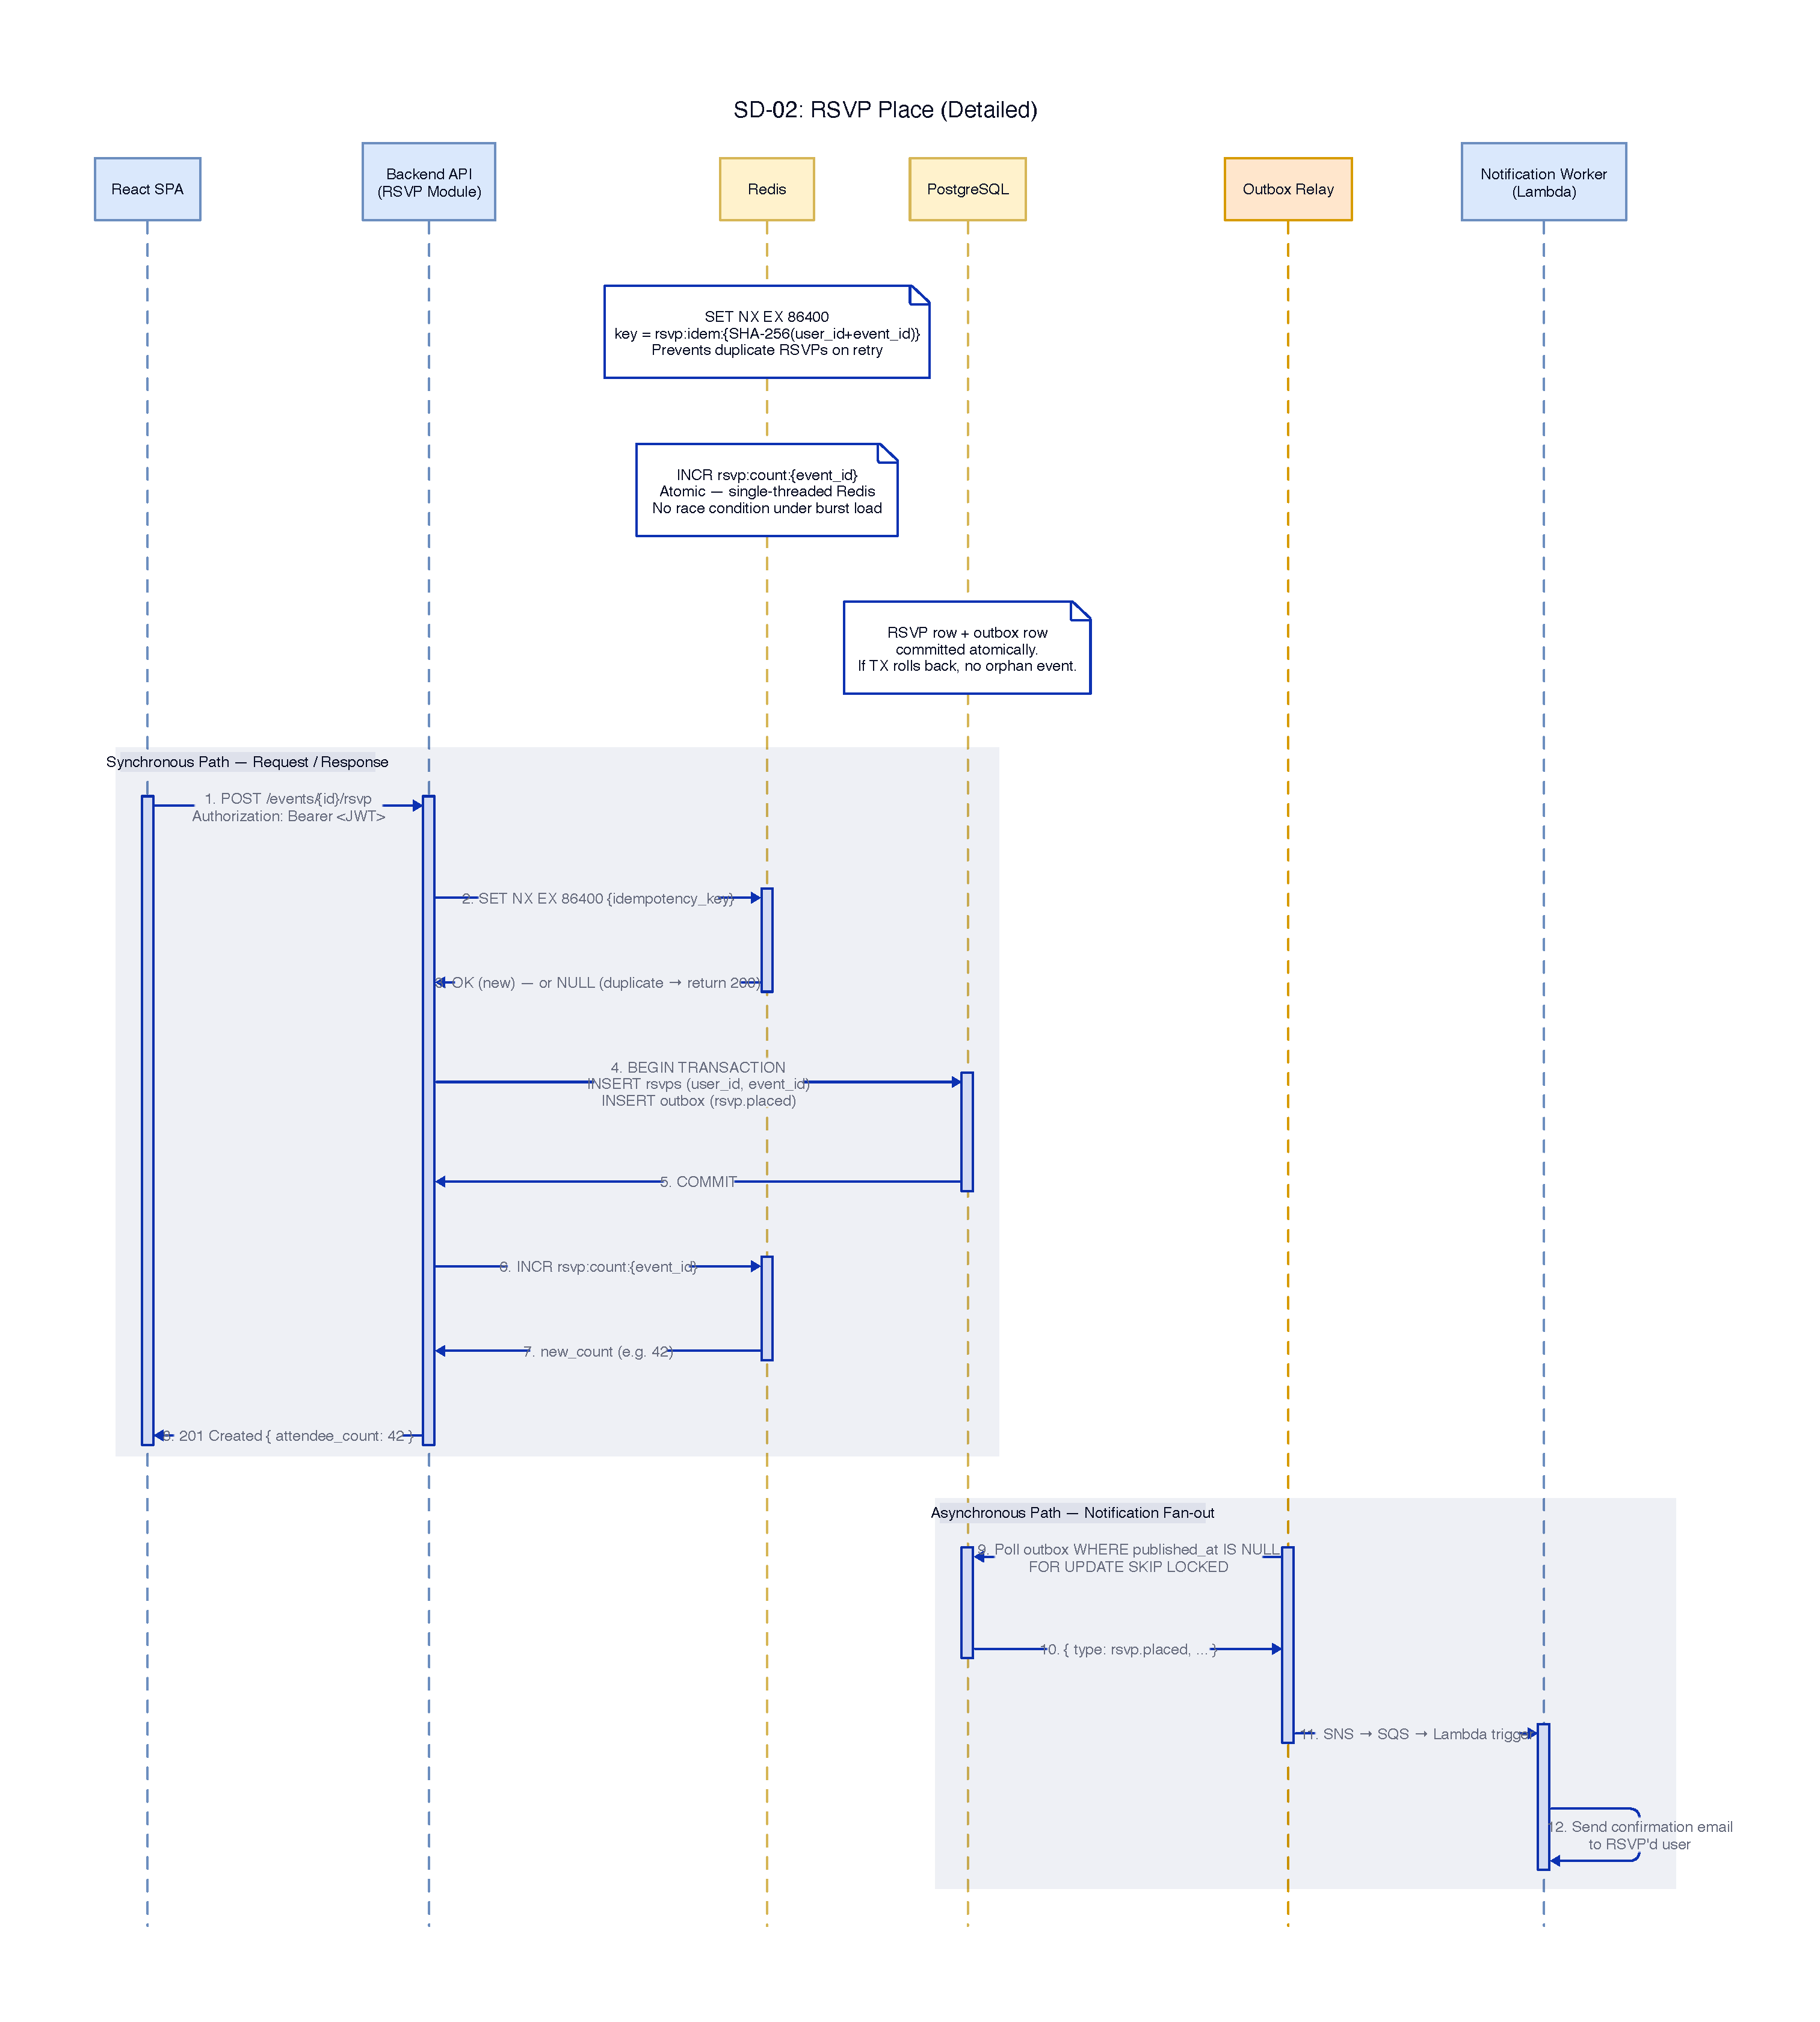
\includegraphics[width=\linewidth,height=0.85\textheight,keepaspectratio]{figures/seq_rsvp.pdf}
  \caption{Sequence diagram for RSVP placement, showing the strict order of operations: event lookup, authorisation, idempotency check, counter seed, row insert, transactional outbox, commit, then cache increment (ADR-0005).}
  \label{fig:seq:rsvp}
\end{figure}

\clearpage

\subsection{Sequence Diagram: Authentication Flow}
\label{app:seq:auth}

\begin{figure}[H]
  \centering
  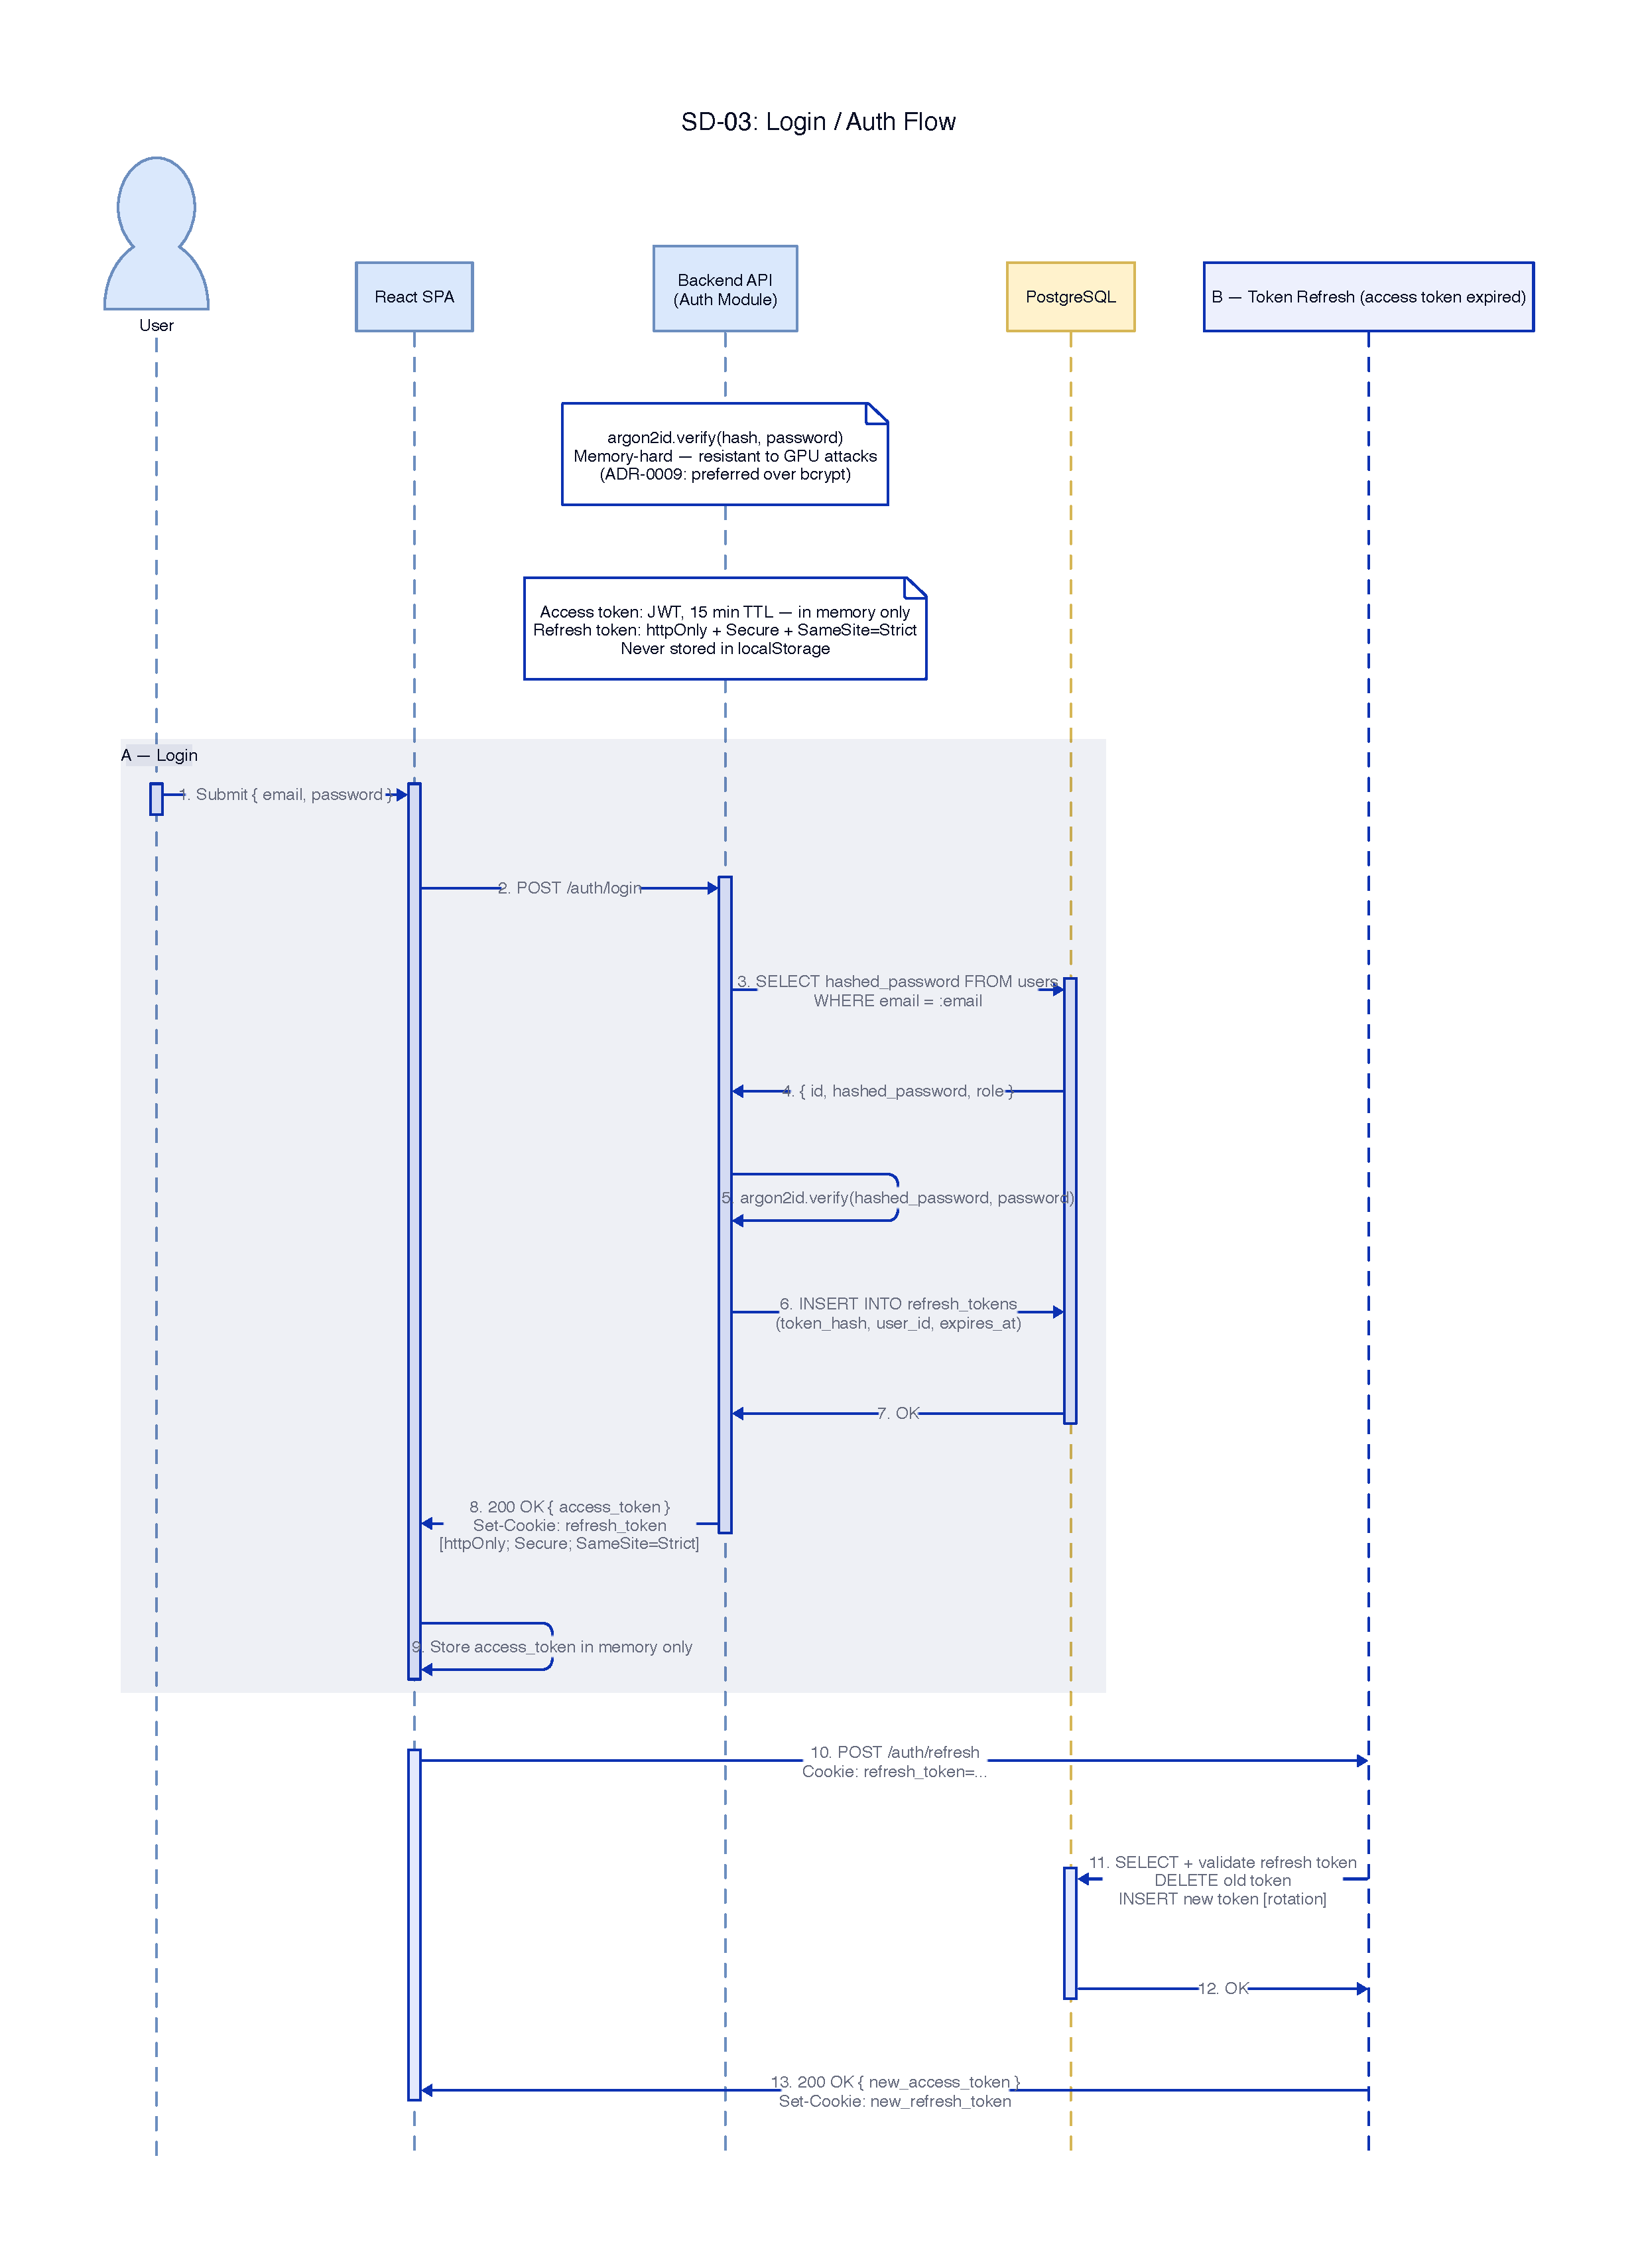
\includegraphics[width=\linewidth,height=0.85\textheight,keepaspectratio]{figures/seq_auth.pdf}
  \caption{Authentication sequence covering registration, login with short-lived access token and rotating refresh token, and token refresh (ADR-0014).}
  \label{fig:seq:auth}
\end{figure}

\clearpage

\subsection{Sequence Diagram: Visibility Transition}
\label{app:seq:visibility}

\begin{figure}[H]
  \centering
  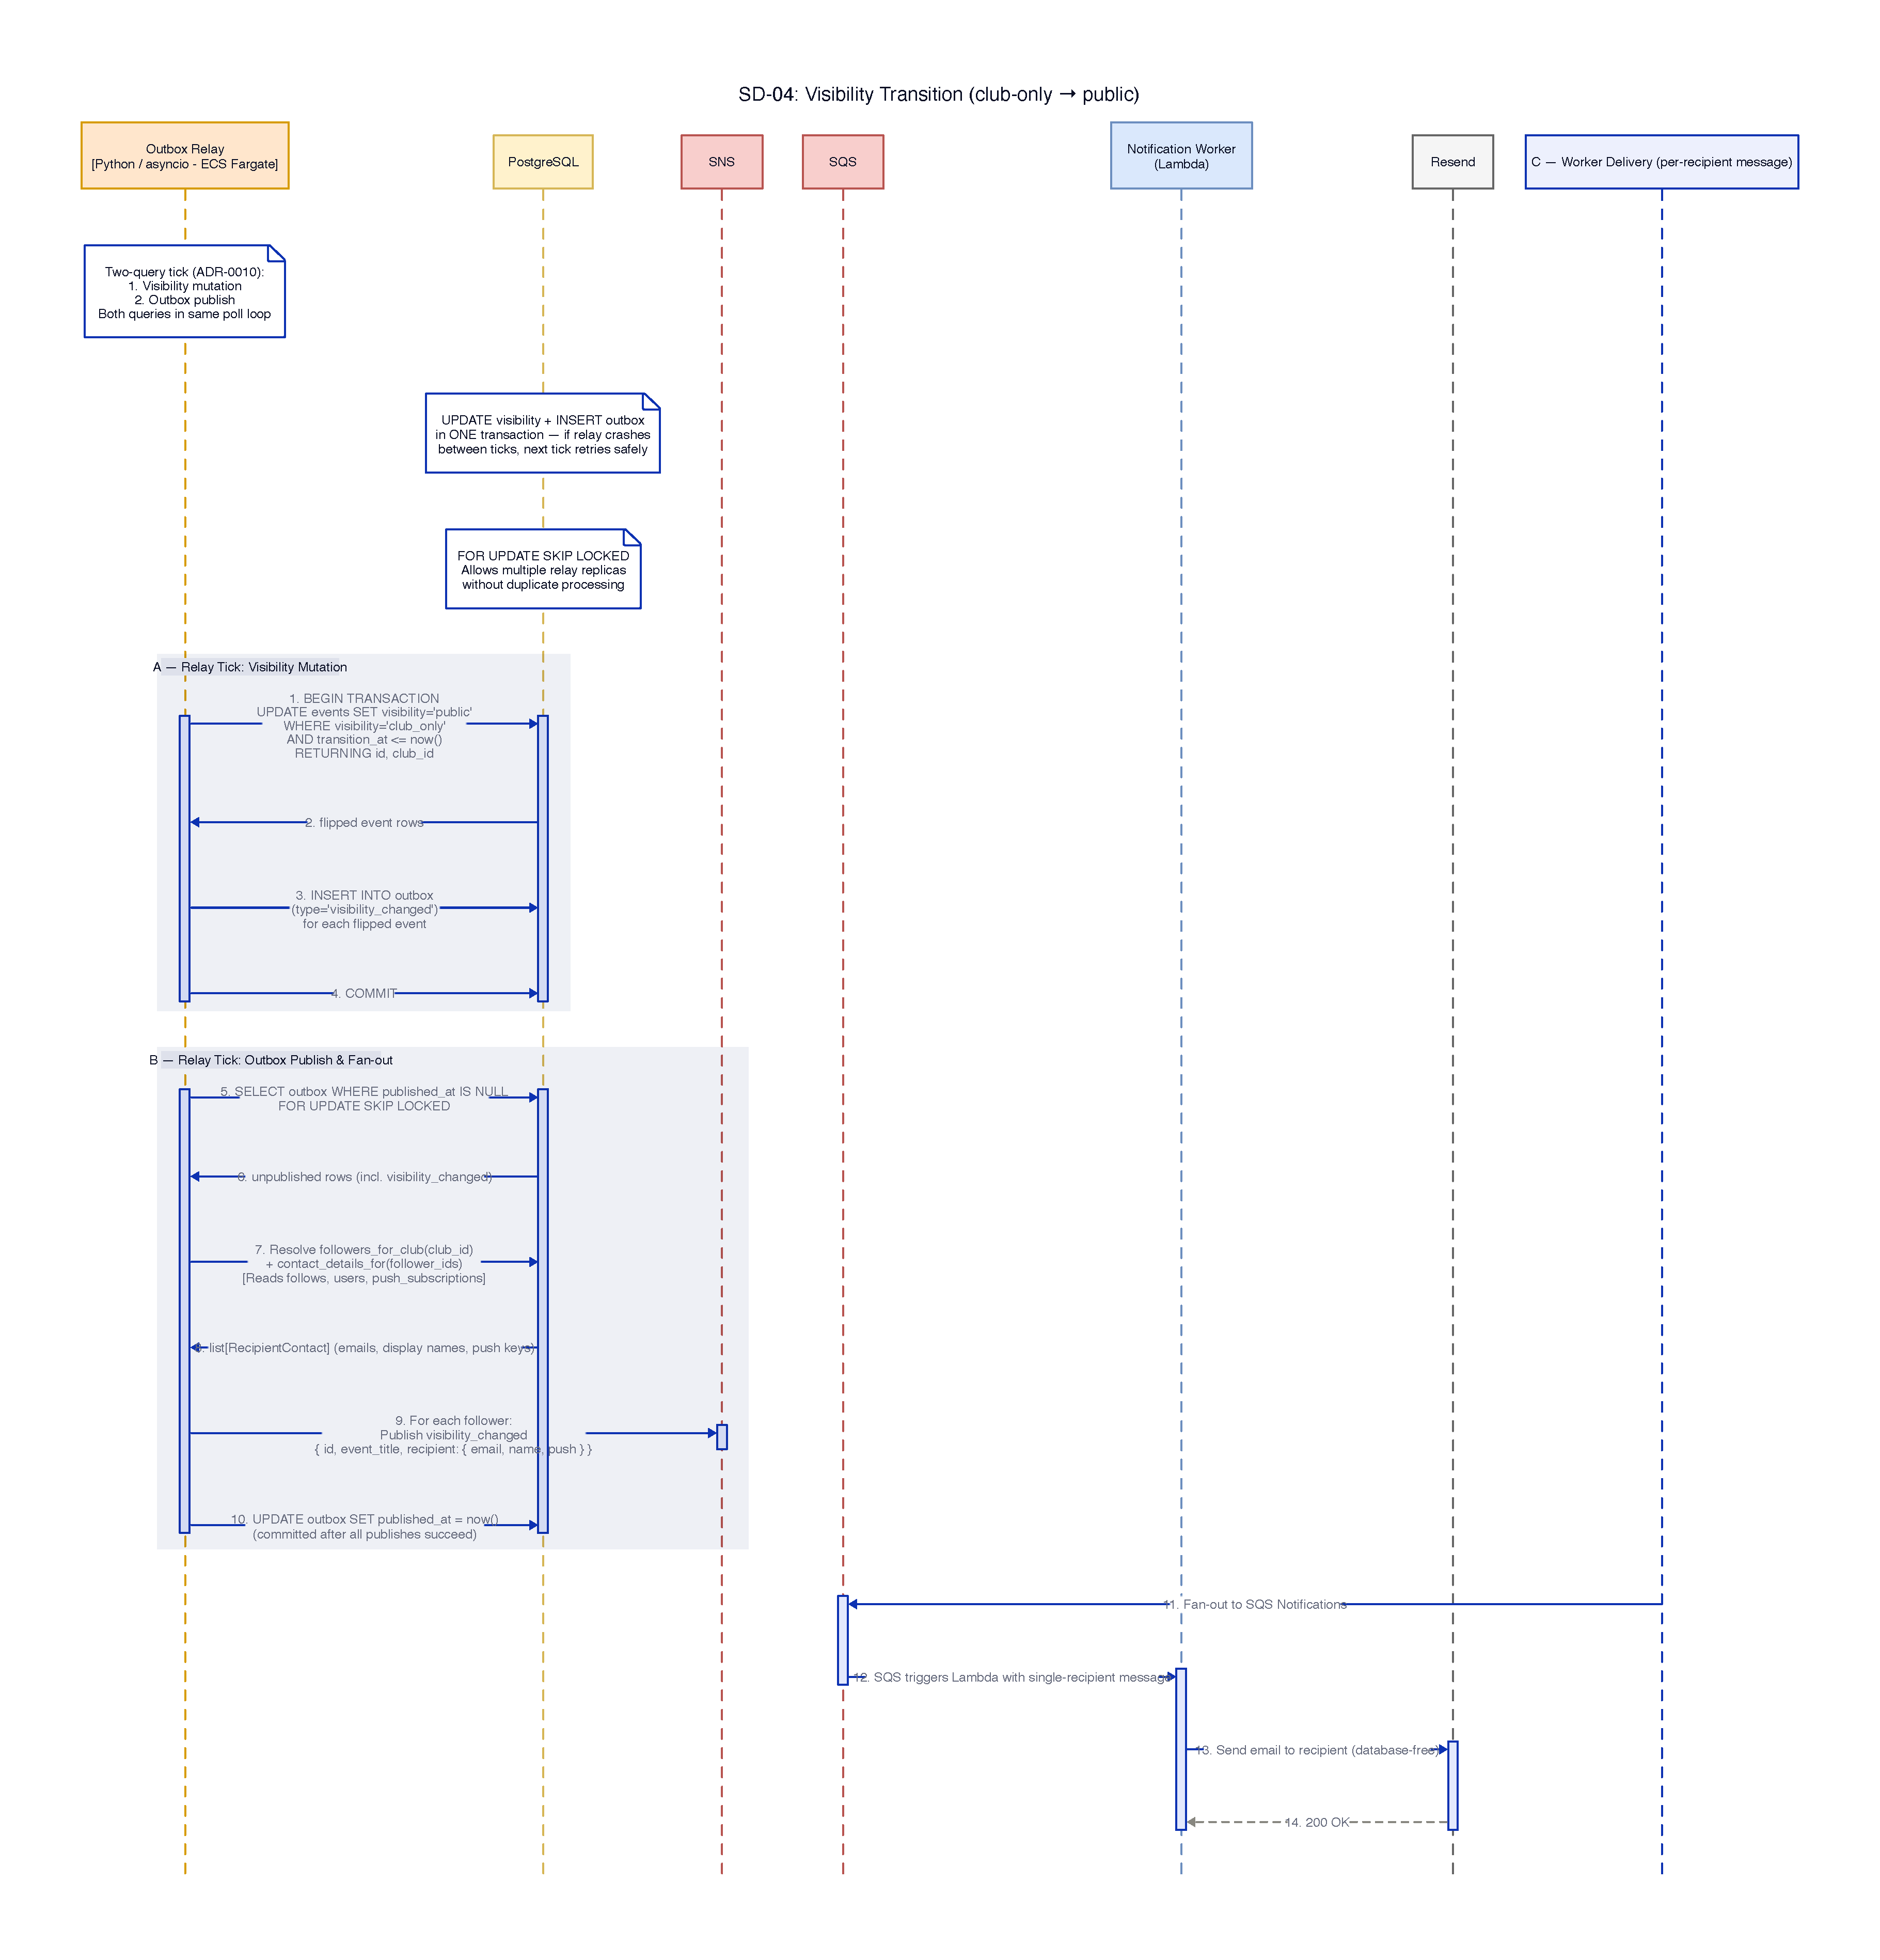
\includegraphics[width=\linewidth,height=0.85\textheight,keepaspectratio]{figures/seq_visibility.pdf}
  \caption{Visibility transition flow: the relay flips club-only events to public at their scheduled time, then publishes a \texttt{visibility\_changed} event through the outbox pipeline (ADR-0010).}
  \label{fig:seq:visibility}
\end{figure}

\clearpage

\subsection{Sequence Diagram: Browse Events}
\label{app:seq:browse}

\begin{figure}[H]
  \centering
  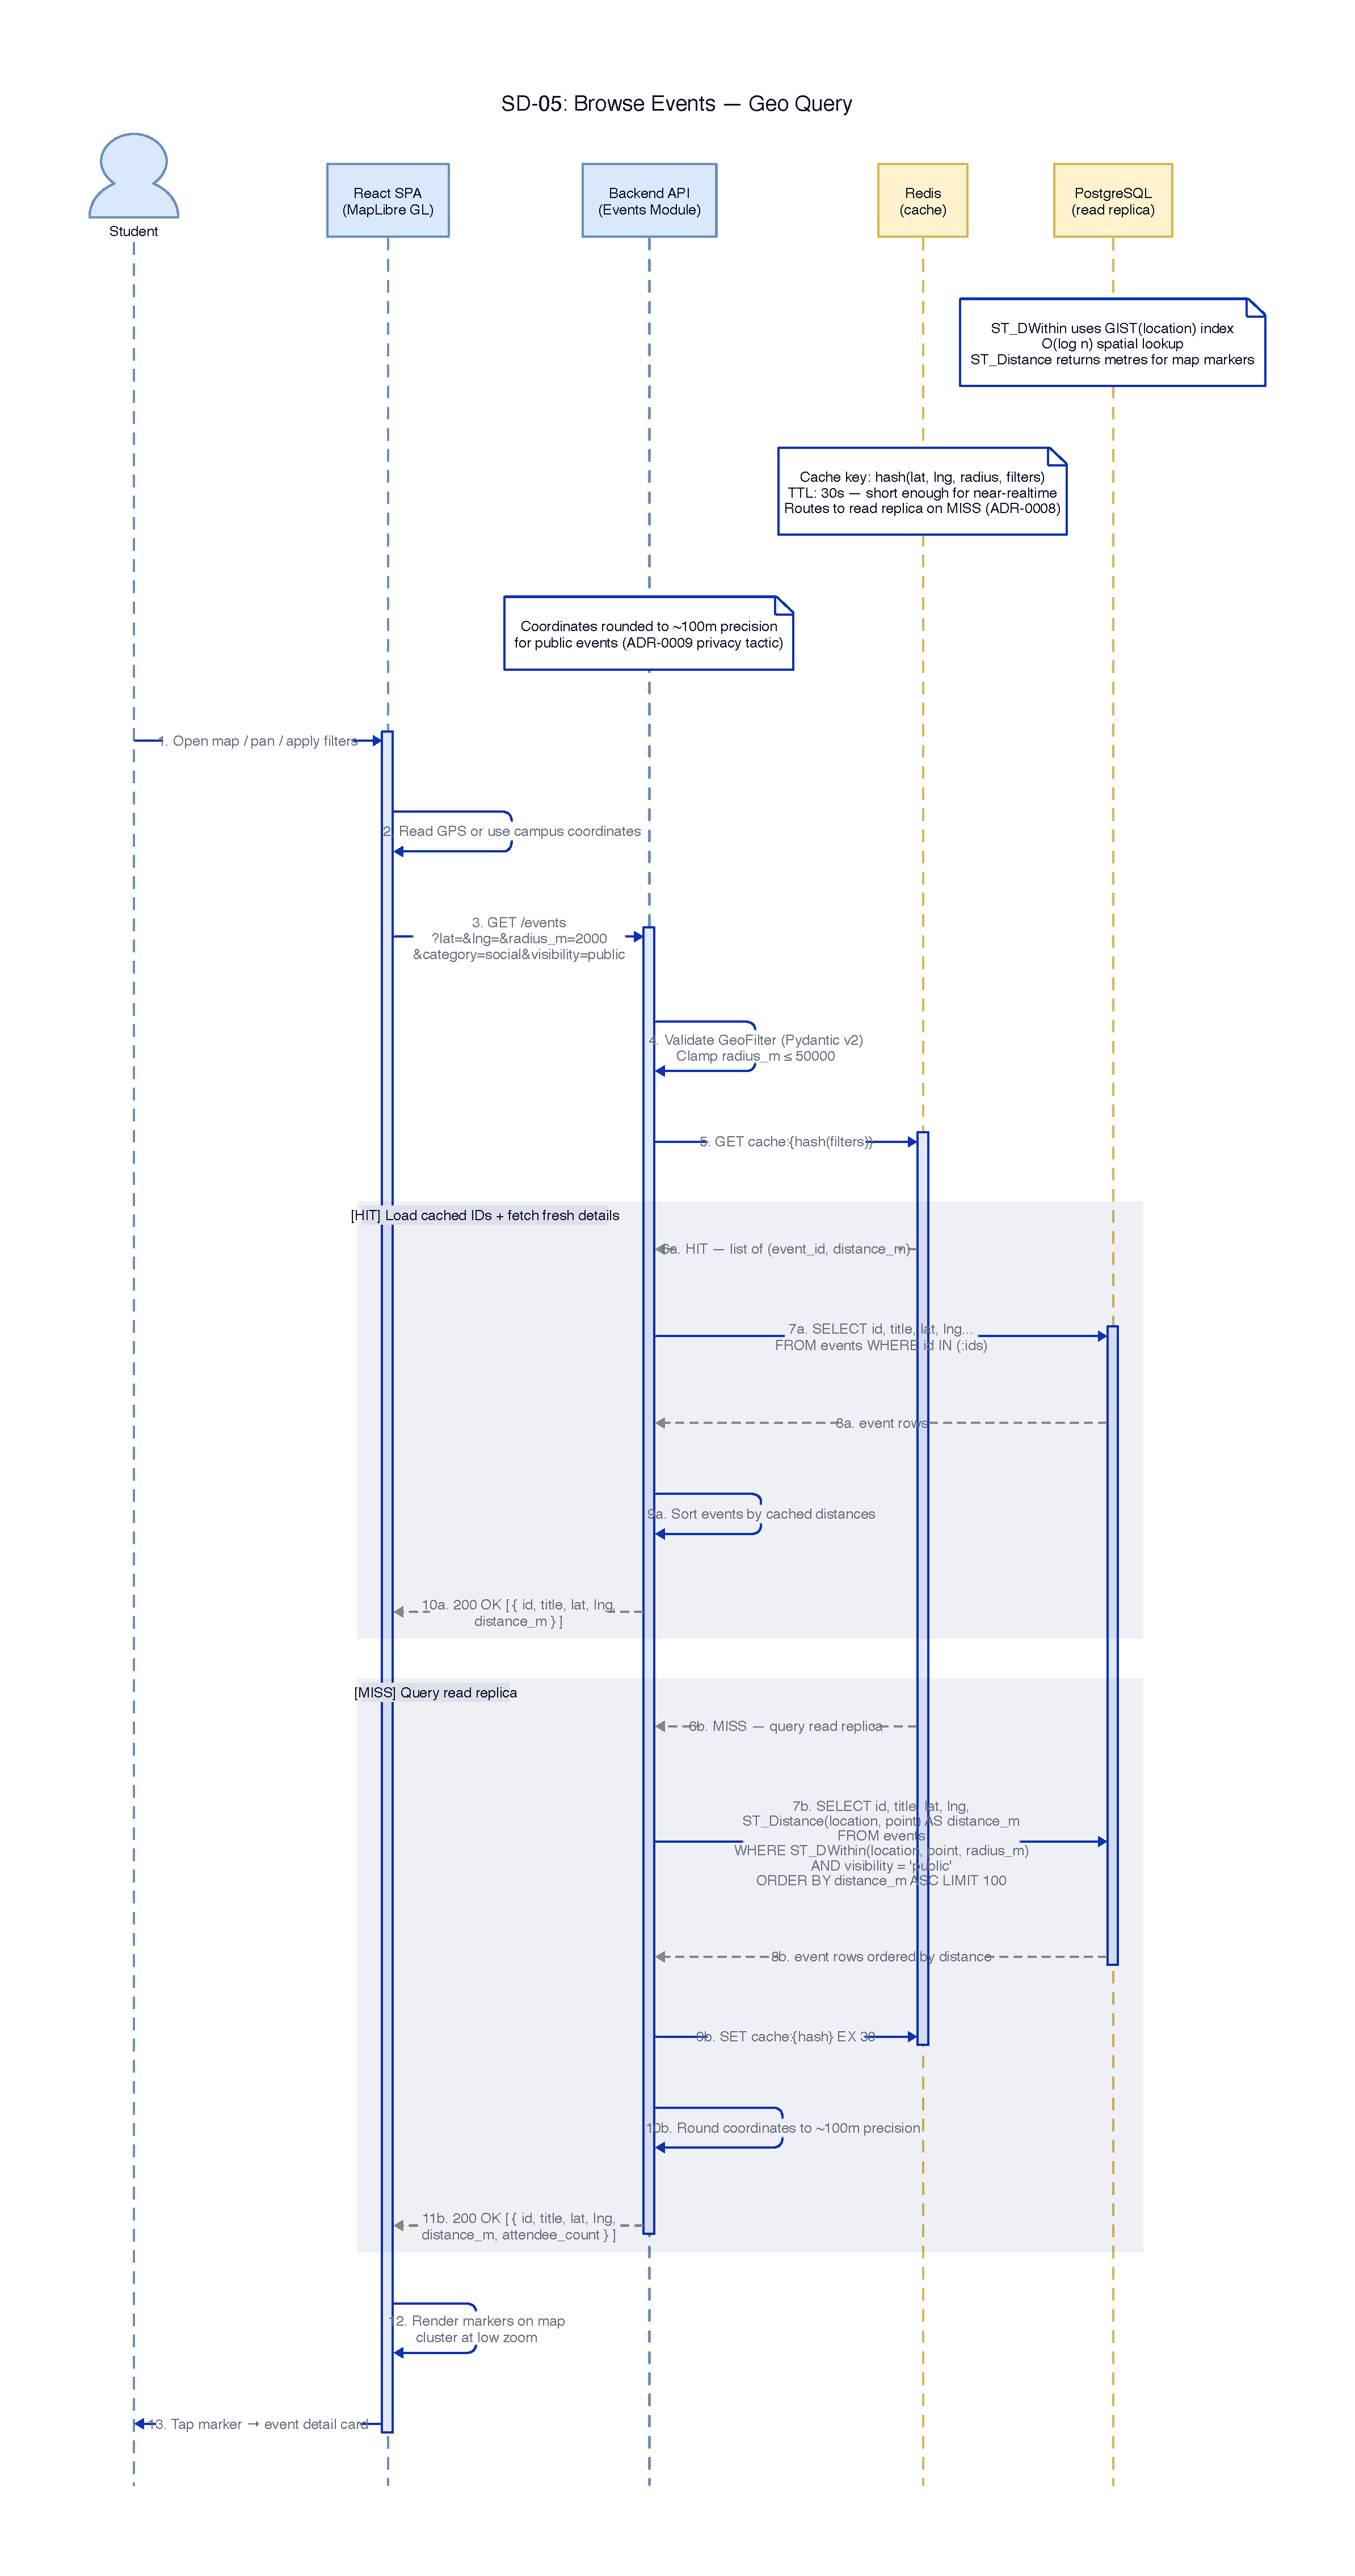
\includegraphics[width=\linewidth,height=0.85\textheight,keepaspectratio]{figures/seq_browse.pdf}
  \caption{Event browsing flow: a student browses public events on the map with geo-radius and category filters, with queries served from the read replica.}
  \label{fig:seq:browse}
\end{figure}

\clearpage

\subsection{Sequence Diagram: Calendar Export}
\label{app:seq:calendar}

\begin{figure}[H]
  \centering
  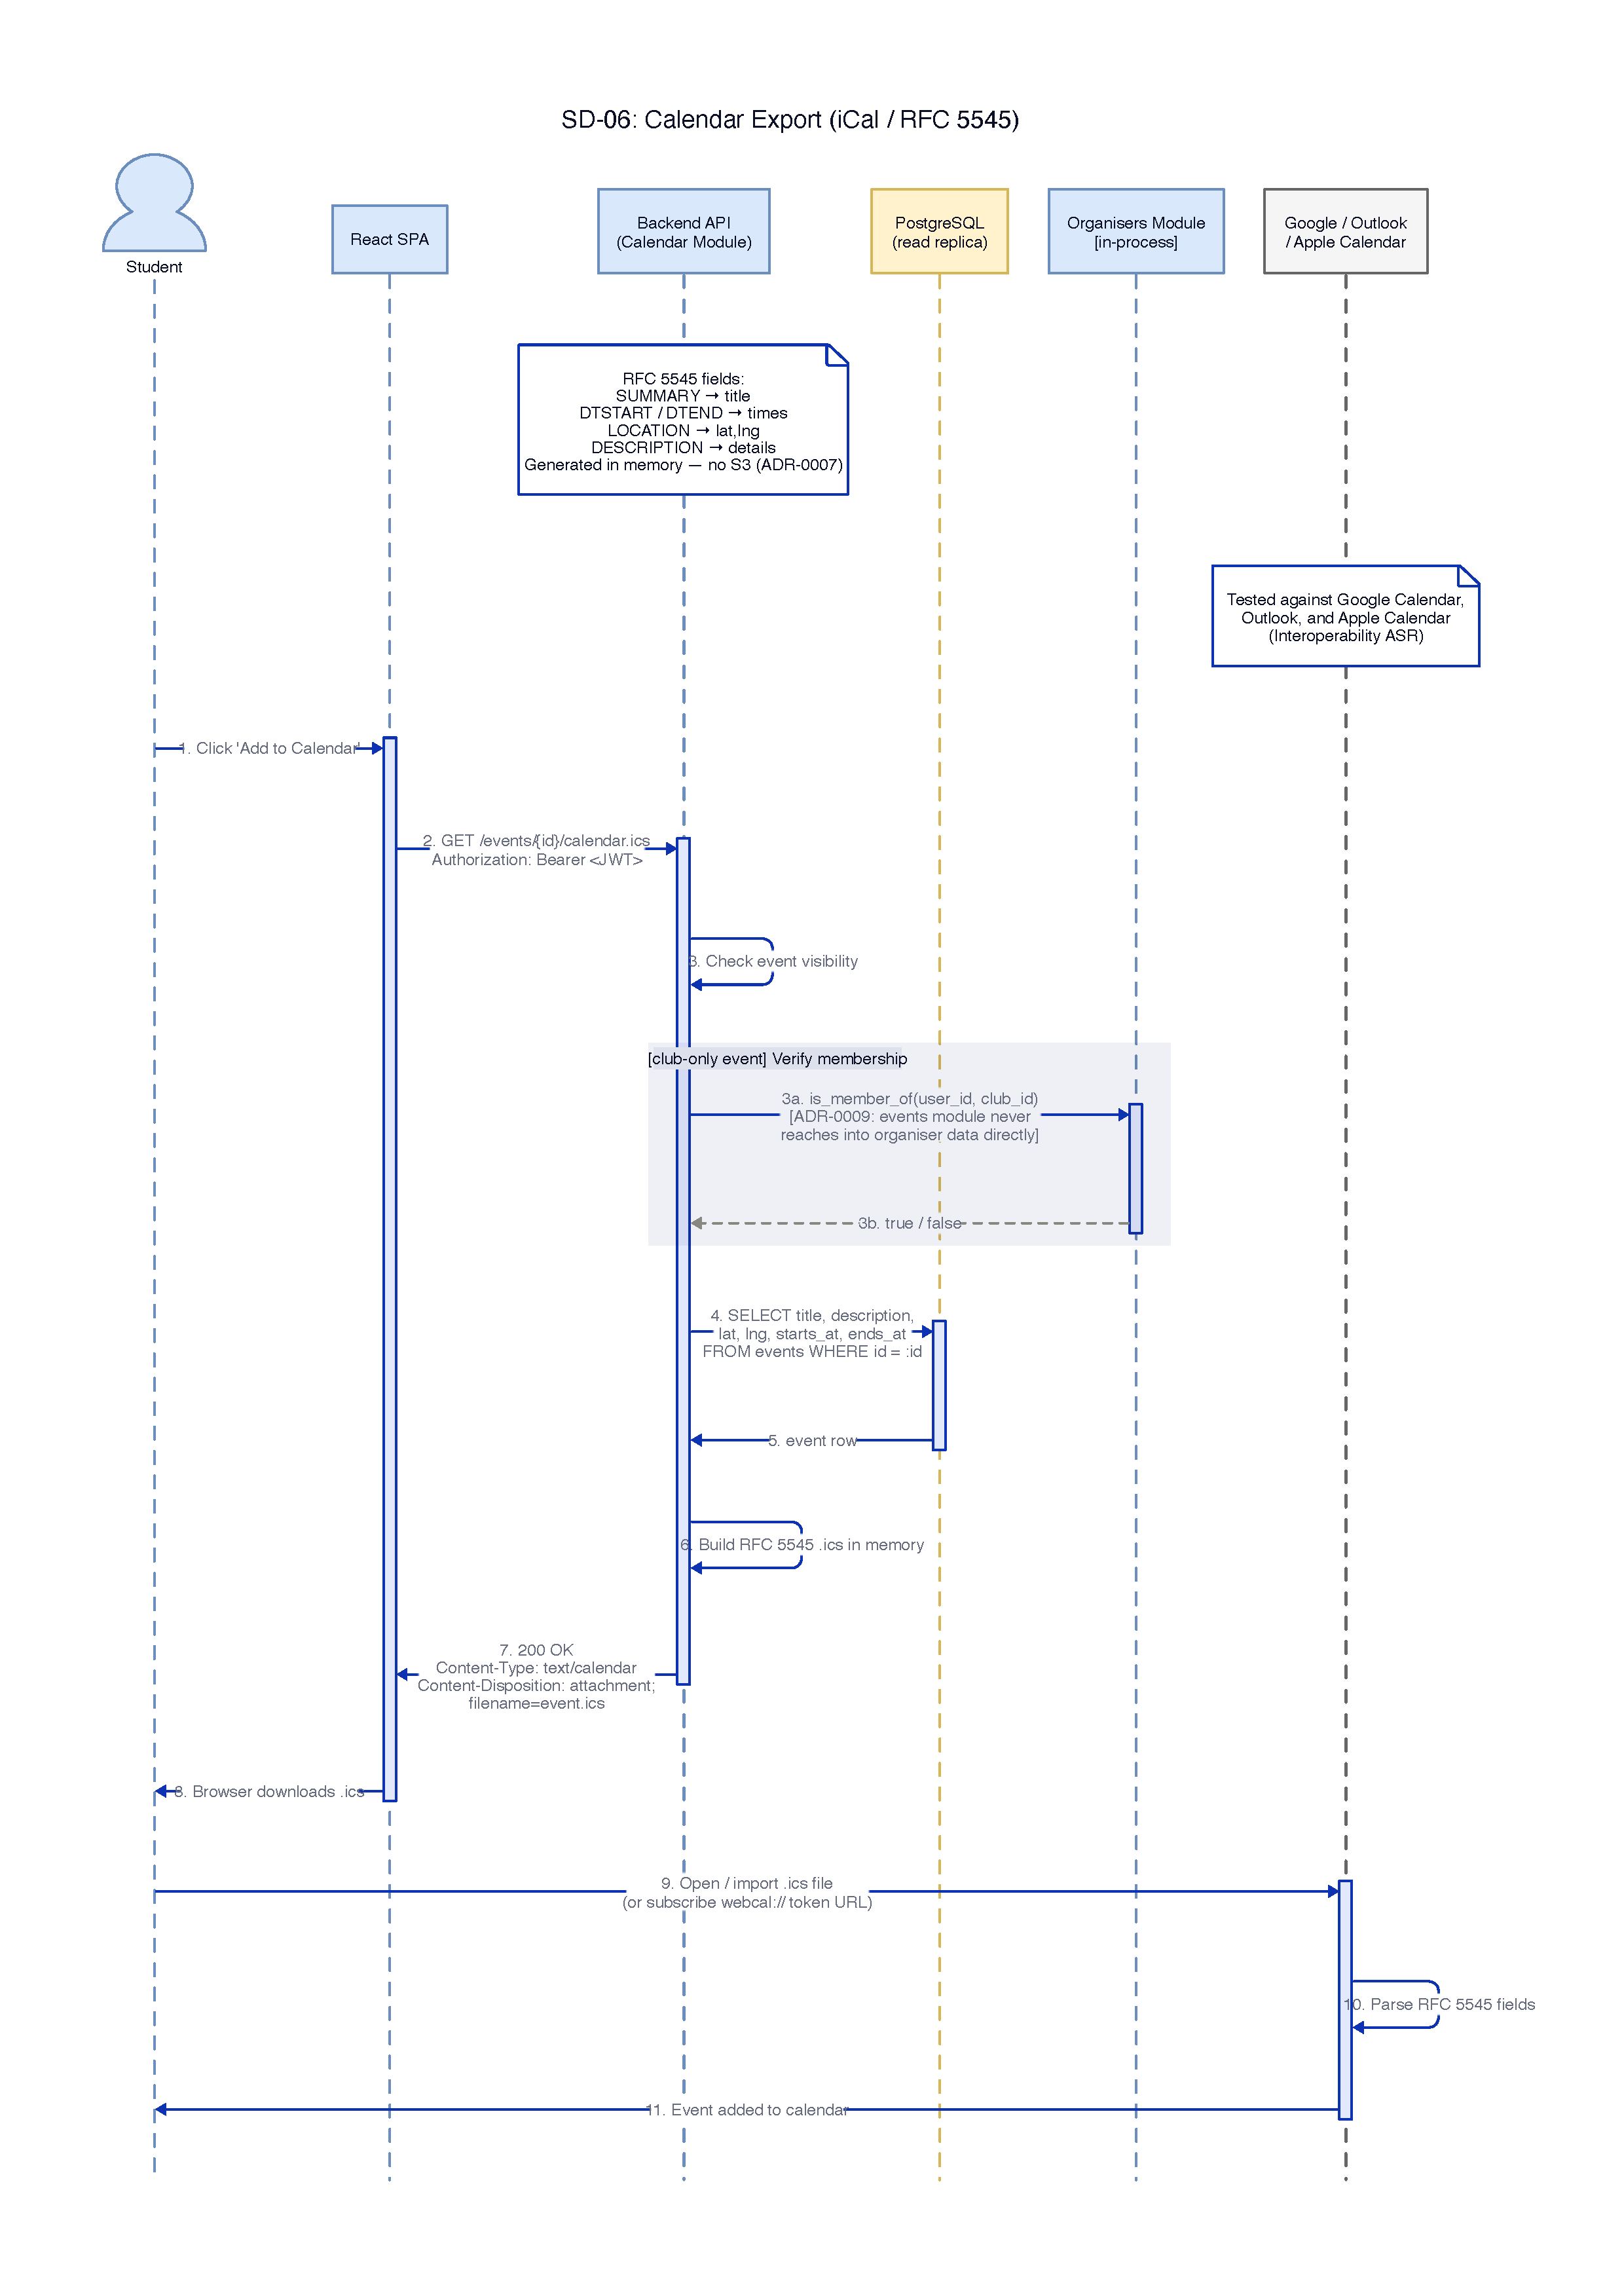
\includegraphics[width=\linewidth,height=0.85\textheight,keepaspectratio]{figures/seq_calendar.pdf}
  \caption{Calendar export flow: a user generates an RFC 5545 iCalendar feed and imports it into an external calendar client.}
  \label{fig:seq:calendar}
\end{figure}

\clearpage